\chapter{Related Work}
\label{chap:Related Work}

Before we can start to investigate the usage of machine-learning based interpolation techniques in the context of urban climate data, we first need to understand what UHIs are and how they can be classified and detected to define requirements for the ML models later. Especially in the context of smart cities with new possibilities such as sensor networks, we need to understand how urban climate data can be collected and what challenges arise such as spatial and temporal data availability, data quality and more. Due to the complexity of the urban climate~\cite{oke2006guideline}, special domain knowledge is needed to understand the data and the underlying processes.
Finally, we need to get an understanding of existing interpolation techniques, traditionally in the form of regression analyses or in the context of climate data, geostatistical models, to define a baseline for the evaluation of ML-based models.

\section{Urban Heat Islands (UHI)}

UHIs have been the centre of a lot of attention for quite some time in the scientific community. As early as 1833, with the research of Luke Howard in London who observed higher temperatures inside London than in surrounding areas~\cite{howard1833climate}, UHIs have seen a steadily increase in scientific contributions. The term \textit{Urban Heat Island} was first introduced in the 1940s~\cite{balchin1947micro}. The recording and investigation of UHIs has seen mayor steps since the begin of modern climatology, also known as the Sundborg's era beginning with Sundborg's 1951 classic heat island study of Uppsala~\cite{sundborg1951climatological}. UHIs occur in many cities around the globe~\cite{peng2012surface} in different climatic zones, during different times of day and in different intensities.\\
UHIs are so important, because heat related deaths are rising across the globe~\cite{kovats2008heat} and extreme heat waves are projected to occur more often and extreme with the ongoing climate change~\cite{lorenz2019detection}. Heat also has significant impact on human performance~\cite{kjellstrom2016heat}, mental health~\cite{obradovich2018empirical}, or can disrupt sleep~\cite{obradovich2017nighttime} and causes other issues such as overheating that causes urban infrastructure to fail, decreased air quality and low outdoor thermal comfort levels~\cite{stone2013climate}.

\subsection{UHI Classification}

UHIs can be classified in many ways. Typically, there is a horizontal classification, defining the superficial extension of the UHI from micro-, to local- to meso-scale, and a vertical classification, defining in which vertical layer of the urban area the heat island is observed. To better understand these scales and the anatomy of the planetary/urban boundary layer, Figures~\ref{fig:mesoscale boundary layer},~\ref{fig:localscale boundary layer}, and~\ref{fig:microscale boundary layer} show a detailed view of the meso-, local- and micro-scale of the urban climate respectively, as illustrated by Oke 2006~\cite{oke2006guideline}.

\begin{figure}[h]
    \centering
    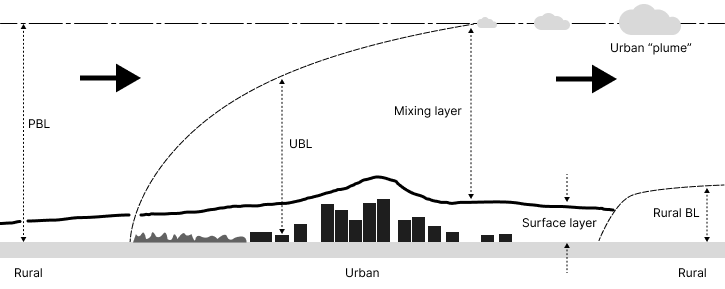
\includegraphics[width=\textwidth]{images/Mesoscale Boundary Layer.png}
    \caption{Mesoscale view of the urban climate, redrawn from~\cite{oke2006guideline}}
    \label{fig:mesoscale boundary layer}
\end{figure}

The mesoscale, as depicted in Fig~\ref{fig:mesoscale boundary layer}, spans the whole urban environment of a city, typically tens of kilometres. There are several boundary layers, that comprise different scales. The planetary boundary layer (PBL)~\cite{wyngaard1985structure} is the lowest layer of the Earth's atmosphere and spans from the surface to a height of several hundred meters up to several kilometres. It is characterised by the turbulent mixing of air, forming wind currents, that are mayorly influenced by the underlying surface.

\begin{figure}[h]
    \centering
    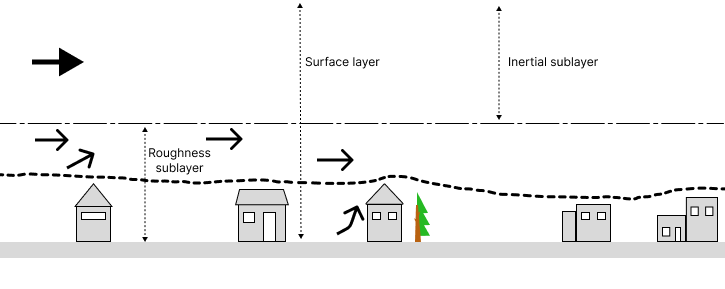
\includegraphics[width=\textwidth]{images/Localscale Boundary Layer.png}
    \caption{Localscale view of the urban climate, redrawn from~\cite{oke2006guideline}, (Todo finish)}
    \label{fig:localscale boundary layer}
\end{figure}

The local scale is situated closer to the surface and contains landscape features such as topography but does not yet include microscale effects. At this layer, the underlying microclimatic effects in form of fluxes mix to form a more average and representative view of the source area, typically at the scale of one to several kilometres. This layer is monitored by weather stations that are located at/or slightly above the canopy height.

\begin{figure}[h]
    \centering
    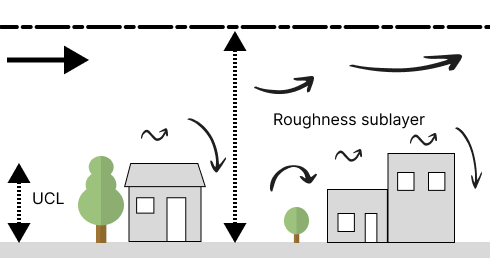
\includegraphics[width=\textwidth]{images/microscale boundary layer.png}
    \caption{Microscale view of the urban climate, redrawn from~\cite{oke2006guideline}, (Todo)}
    \label{fig:microscale boundary layer}
\end{figure}

The microscale usually ranges from a neighbourhood scale to individual street canyons or even microclimates created by individual buildings. It is mayorly influenced by the overall energy balance, which is influenced by cloud coverage, solar radiation and more. Single weather stations are not enough to capture the complex microscale~\cite{oke2004siting}, therefore a dense network of sensors closer to the ground is needed to capture the microscale. Additionally, the microclimate is influenced by surface temperature (LST), however the correlation between air and surface temperature varies greatly based on other surrounding influences such as wind velocity or humidity~\cite{stoll1992surface}, especially in cases of extreme temperatures~\cite{good2016situ}. The closer the air temperature is measured to the surface, the more local the measurement, therefore air temperature of the canopy is usually measured at 2m height, so the different energy fluxes have enough time to mix and form a more representative average for a bigger area.\\
Vertically, UHIs can be divided based on these boundary layers into three mayor types~\cite{oke1976distinction, oke2017urban}, namely Boundary Layer Heat Island (BUHI), Canopy Urban Heat Island (CUHI) and Surface Urban Heat Islands (SUHI), corresponding to the boundary layer they can be measured in. Another differentiating factor is the time of day at which UHIs get detected. For example, Steward~\cite{stewart2011systematic} in his review focussed on night-time UHIs, whereas Peng et al.~\cite{peng2012surface} focussed on both day and night-time UHIs.

\subsection{Surface Urban Heat Island (SUHI)}

The land surface temperature (LST) is measured directly at the surface of an object and is the main indicator of the surface urban heat island (SUHI), which can be found in many cities around the globe~\cite{peng2012surface}. Surface temperature, in contrast to air temperature, is measured via remote sensing technologies via satellites. Well-known satellites include MODIS~\cite{didan2021modis} (NASA), Sentinel 3 (ESA), Meteosat (EUMETSAT), Landsat, and more. The different satellite types carry different types of instruments and sensors, that can take various measurements. The used sensor has a mayor influence on the quality of data, e.g.\ resolution via pixel size, robustness against atmospheric influences, ability to handle clouds, and more. In Section~\ref{sec:feature_engineering} we discuss other features next to LST that are available via satellite data.\\
Through the use of satellites, the spatial coverage is great, but raster sizes for older satellites such as MODIS usually range from one to several kilometres, therefore the spatial resolution is not as high. For newer satellites such as Sentinel 2 and Landsat, pixel sizes are improved significantly from 10m to 50m, however complementary data such as derived vegetation indexes are usually not available as precomputed values, adding additional work to the data retrieval process, as later discussed in Section~\ref{subsec: remote sensing}.
Additionally, weather satellites usually orbit earth to cover wide areas and are not geostationary, therefore only taking measurements a maximum of 1 to 2 times a day, up to every 16 days or even only once a month, depending on the orbit. As a result, the temporal resolution is quite low and especially in the case of UHI detection, this could mean that the satellite misses the peak of the UHI for a given day or even misses the UHI completely. Another downside is the general inability to take LST measurements through clouds, therefore even if the satellite passes over during a UHI, if there are clouds, the UHI cannot be measured. To alleviate the problem there are new methods such as estimating LST based on emitted radiation from clouds~\cite{zhang2015estimation}, however they also have their limitations. Lastly, LST and air temperature are not the same and can vary greatly, especially in extreme heat events~\cite{good2016situ}.\\
To conclude, SUHI analysis can be a good indicator that there is a UHI phenomenon present in a city and can generally direct further research, however it lacks the temporal resolution to be used for real-time UHI detection and is not able to capture microscale effects of the UHI~\cite{voogt2003thermal, voelkel2017towards}.

\subsection{Canopy Urban Heat Island (CUHI)}

The canopy UHI is measured in the canopy boundary layer several meters above ground slightly below or on the average roof layer of the surrounding buildings, as seen in fig.~\ref{fig:microscale boundary layer}. The primary measurement in the canopy is air temperature, which is used to measure the urban heat island intensity (UHII)~\cite{oke1973city}, the most used way of describing the heat island magnitude~\cite{kim2021urban}.\\
Since the beginning of modern climatology, mayor progress has been made in this research field, but methodologies and scientific rigor in CUHI research still seems to be lacking, as discussed by Stewart in 2011~\cite{stewart2011systematic}. Stewart found, that over 54\% of CUHI research was lacking proper methodologies or had other shortcomings such as a lack of site descriptions, where sensors were placed, or the disregard of non-urban factors such as local weather phenomena. In response, progress has been made in recent years by improving methodologies and ensuring correct measurements of climate-related data and study design and execution through various guidelines~\cite{oke2006guideline}, especially in urban settings, that require special care due to the huge number of possible influences on local recording sites.\\
Additionally, the UHII is highly related to other climatic factors such as wind, cloud cover, and precipitation and is tightly linked to the selection of the recording site~\cite{fenner2019contrasting}, therefore such factors need to be considered when measuring the UHII.\\
Compared to LST, TA is measured in situ via weather station networks or other types of sensor networks. Provider for PWS and temperature sensor networks are further discussed in Section~\ref{sec: private weather station network providers}.

\subsubsection{Shared UHI Challenges}

Some shared challenges for all types of UHI include: 1. Define what \textit{urban} means in the context of UHIs~\cite{stewart2009newly}. The term urban is widely used to identify areas that are more densly populated than the surrounding rural areas. Having this distinction between urban and rural~\cite{lowry1977empirical} helped researchers to better define the UHI magnitude, but this simple distinction also leads to problems~\cite{stewart2011systematic}. The problem lies in the fact that there is no clear border between urban and rural areas, but a fluent transition. Especially for larger metropolitan areas, like Tokyo, the urban area could span 10s to 100s of kilometres, making the collection of reference rural temperatures hard. The reference rural temperature has a direct influence on the UHI magnitude, which is `the most widely recognized indicator of city climate modification in the environmental sciences'~\cite{stewart2009newly}. As a solution, different classification into local climate zones were proposed~\cite{stewart2012local, stewart2009newly}, that classify areas based on surface roughness, building densities, building heights etc. 2. Measuring the influence of other local urban or meteorologicalphenomena on the temperatures collected. The urban climate is extremely complex, due to many different influences, such as anthropological energy, heat dissipated from ACs, vehicles, and more. Additionally, the urban climate is also influenced by surrounding regional/meso-scale climate phenomena such as storms, valleys, mountains, large waterbodies, coastlines, and more. In Section~\ref{sec:feature_engineering}, we talk about potential features to capture the local urban climate.

\section{Smart Cities}

Smart Cities offer many new possibilities, enabling new ways of communication and sensing applications. To find out how Smart Cities are structured and how applications could take advantage of data provided by a Smart City, we look at its general architecture.
The most generalised architecture of a smart city consists of four layers, the sensing layer, transmission layer, data management, and application layer~\cite{silva2018towards}. In this work, we focus on the sensing layer, dealing with topics such as correct sensor placement and underlying sensor footprints, and the application layer, which accesses available data via data management services to provide additional services to the city and its citizens. For the data transmission and data management layers, there already exist different technologies and service offerings, that aim at solving the underlying problems, e.g.\ network bandwidth, network availability, sensor discoverability, handling the massive amounts of data that is already or will be collected in the future, and many more. For the communication and discovery of sensor nodes, one solution could be SkipNet~\cite{harvey2002skipnet}, an overlay network focused on discoverability while also protecting privacy, with which the data transportation layer could be designed as a peer-to-peer (P2P) network. Other research focuses on the data accessibility and discoverability, by making data accessible for everyone, not only for economic partners in a closed-off system. Examples would be the Smart Networks for Urban Citizen Participation (SANE) initiative~\cite{bornholdt2019sane}, which could provide crowd-sourced distributed air temperature sensing with a framework to make sensors searchable and subscribable, allowing real-time applications by consuming sensor data streams. Figure~\ref{fig:system-architecture-overview} shows how an architecture with SANE could look like.\\
In connection to this work, ML-based interpolation, for example for air temperature, could be used to augment Smart City applications by supplying data for sensor locations while a sensor is offline, or by turning discrete sensor readings into a temperature map that could be used by researchers for further heat related analysis or by decision makers to inform and visualise heat stress in a city.\\

\begin{figure}[h]
    \centering
    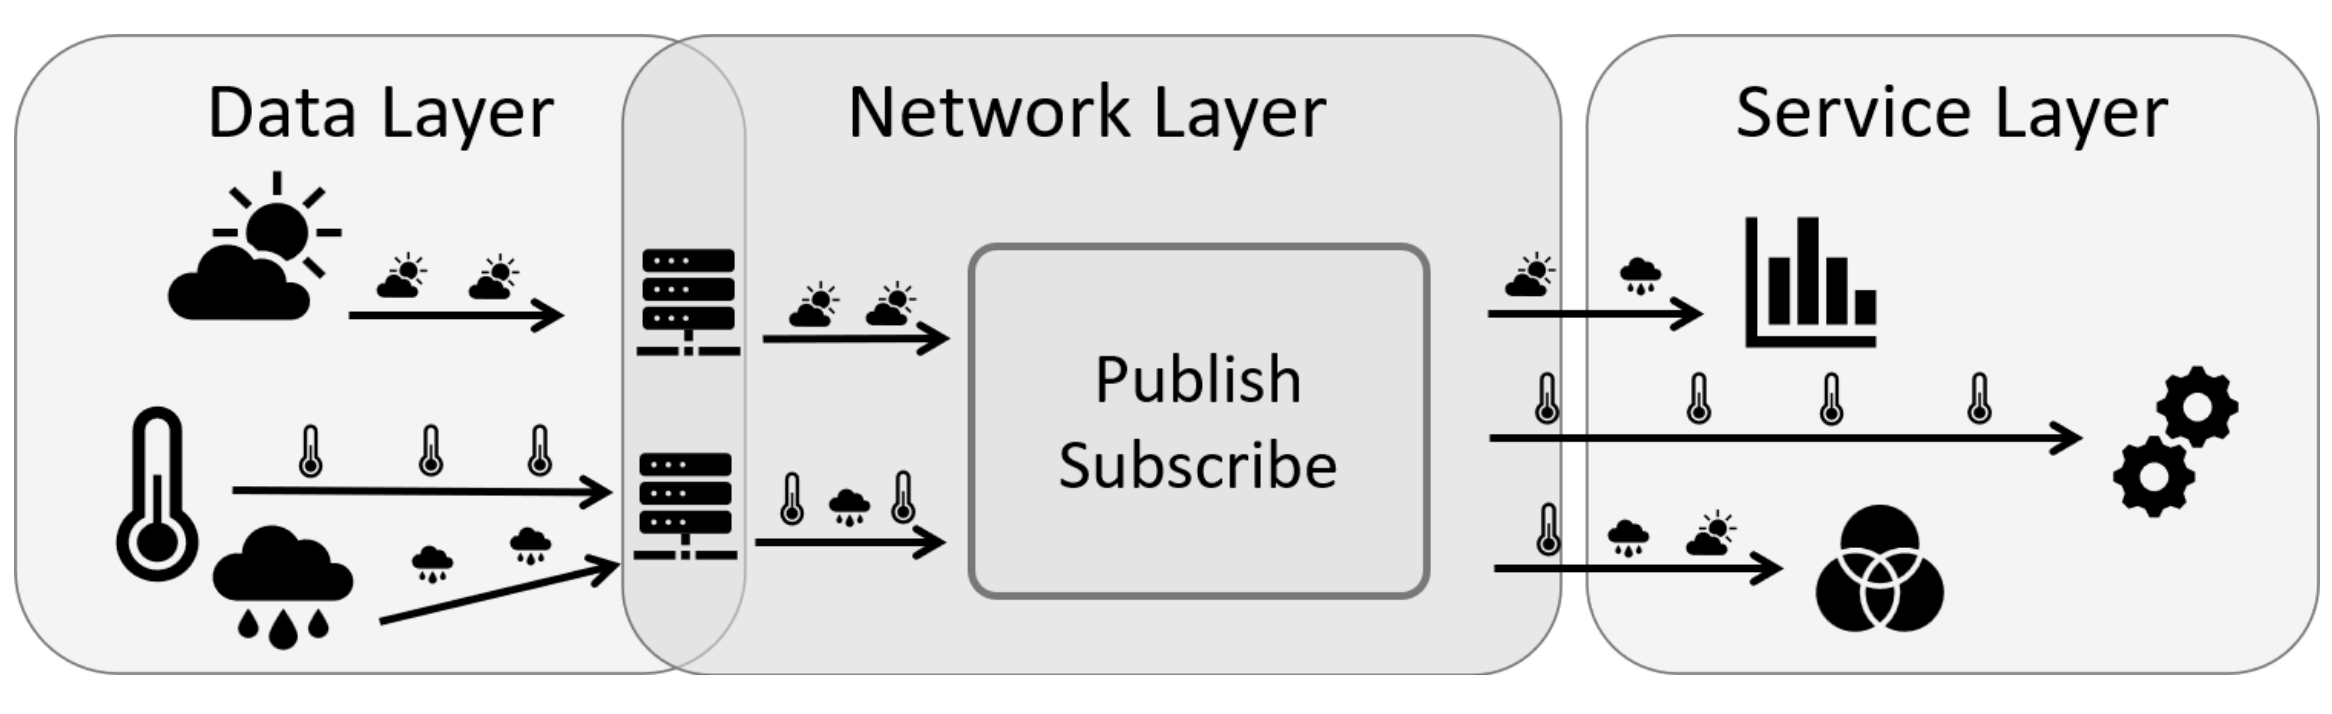
\includegraphics[width=\textwidth]{images/expose-system-architecture.png}
    \caption{In the data layer (left), a wide variety of environmental data is collected with the help of multiple sensors. These are connected to their citizen-owned local base stations, which manage access rights and forward collected data to subscribed services (right) via the decentralized publish-subscribe in the network layer (centre).}
    \label{fig:system-architecture-overview}
\end{figure}

\subsection{Sensing Layer}

The goal for the sensing layer is to monitor the surrounding environment and capture key data for further analysis and decision making. It consists of many different types of physical and virtual sensors. The first group of sensors are the physical sensors, which are placed directly inside the environment. Wireless sensor networks (WSN)~\cite{dargie2010fundamentals} have seen a lot of attention for many different applications such as `military sensing, physical security, air traffic control, traffic surveillance, video surveillance, industrial and manufacturing automation, distributed robotics, environment monitoring, and building and structures monitoring'~\cite{chong2003sensor}. The challenges for WSNs primarily depend among other things on the deployment. An ad-hoc WSN has energy and bandwidth constraints due to the usage of batteries as power sources.
In contrast, sensors that are permanently installed, either stationary or on a moving target, and connected to a constant power source don't have these constraints. This approach could be used for smart cities to reduce waste and guarantee representative measurements via correct sensor placement. In the case of stationary sensor networks though, the initial deployment and following maintenance cost can be substantial, as seen by the Birmingham Testbed~\cite{chapman2015birmingham}. If the cost is however distributed across many by following a crowd-sourcing approach, e.g.\ crowd-sensing via PWS, larger networks could be maintained, but there are also new challenges introduced by running sensor networks by non-professionals~\cite{meier2017crowdsourcing}.\\
In recent years, low-cost sensors (LCS) in combination with sensor networks have enabled fine-granular real-time monitoring of urban environments~\cite{grimmond2006progress, rundel2009environmental}, although the quality of individual low-cost sensors can be questionable~\cite{castell2017can}. Especially PWS data has been used to augment weather data from traditional weather monitoring networks from official weather services~\cite{hahn2022observations}. In general, LCSs can improve data availability and support analysis, but do not substitute well-calibrated reference instrumentation~\cite{lewis2018low}.

\subsubsection{Stationary Sensors}

There are many different types of environmental features that can be measured directly inside an urban area. The types of measurements that can be observed are among others: air temperature, humidity, atmospheric pressure, reactive gaseous air pollutant (CO, NOx, O$_3$, SO$_2$), particulate matter (PM), greenhouse gases (CO$_2$, CH$_4$), precipitation, solar radiation, wind speed and direction, anthropogenic heat, noise, sky-view factor, heat fluxes and many more.
Correlations between these features can vary greatly based on surrounding factors. To better understand these correlations, many empirical studies have studied the influence of meteorological factors on features such as PM~\cite{tai2010correlations}. Additionally, many fields of statistics have specialised on topics such as statistics in climatology~\cite{von2002statistical}, geostatistics~\cite{trangmar1986application} and more.\\
All sensor readings that are taken by physical sensors are singular data points. Additionally, to the type of measurement taken and the actual value observed, physical sensor readings include the physical location of the sensor, e.g.\ latitude, longitude and sometimes altitude, the type of sensor used to take the measurement, and sampling rates. For air temperature, the sampling rate could be an average temperature measured over five minutes, whereas precipitation might be measured by collecting rain for certain periods of time and then measuring the amount of rain collected. The sensor type is important, as different types of sensors can produce different qualities of measurements, e.g.\ LCS have lower accuracy compared to calibrated reference-grade high-cost sensors and might have lower response rates, and perform better or worse based on the meteorological conditions, e.g.\ worse performance at low temperatures, high humidity etc. Due to the placement directly inside the environment, (near) real-time observation and high temporal resolution are generally possible but might be influenced by factors such as network availability. The spatial resolution highly depends on the number of sensors deployed and the correct placement of the sensors. The correct placement has a direct influence on the footprint of the sensor~\cite{leclerc2014footprints} and the representativeness of the measurement taken for the underlying and surrounding area~\cite{oke2006guideline}.\\
One downside of the placement directly in the environment the sensors are observing, is the exposure to environmental influences such as heat, humidity, or pollution, that can decrease the lifetime of a sensor and may require more frequent maintenance or replacement. On example could be that due to pollution in the air, a rain gauge might be cleaned/replaced more often as over time dirt builds up very quickly.

\subsubsection{Mobile Sensors}

Next to stationary sensors such as a PWS, mobile sensors are not bound to one place, but have the ability to move through the environment they are placed in. This increases the spatial coverage at the cost of temporal resolution, as a sensor is not always in the same place. In the context of urban air temperature sensing, LCS could be mounted to moving vehicles such as busses, cars, e-bikes, scooters, and more. This could help improve the spatial coverage of a sensor network. In combination with ML-based interpolation, such moving sensors could be used to create virtual sensors for specific locations, where a ML model learns the relationship between surrounding sensors so that air temperature could be interpolated for times when a moving sensor is currently not at the specific location. In their study, Yang et al.~\cite{yang2019designing} found that randomly mobile sensor networks outperformed completely stationary sensor networks for measuring monthly mean temperatures, however they had higher errors of up to 5°C when measuring daily maximum temperatures. They suggest that hybrid systems with both stationary and moving sensors are more robust in measuring short extreme events such as heat waves.\\
Next to mobile sensor networks, official weather services such as the DWD also do temperature profile measurements~\footnote{\url{https://www.dwd.de/DE/service/lexikon/Functions/glossar.html?lv2=101996&lv3=102106}, \textit{last accessed: 23.08.2023}}, where sensors are mounted to a car to capture air temperature, humidity, wind speed and direction, as well as possibly atmospheric pressure. This data can be used to support research into local climates. Especially interesting for these profile drives are `summer cloud-free and light-windy high-pressure weather conditions, as then temperature differences between the city and the surrounding area become particularly pronounced and temperature-equalising cold air flows reach their greatest intensity.'~\footnote{\url{https://www.dwd.de/DE/forschung/klima\_umwelt/klimawirk/stadtpl/projekt\_warmeinseln/projekt\_waermeinseln\_node.html}, \textit{last accessed: 23.08.2023}}.

\subsection{Application Layer}

The application layer contains services which utilize data provided by the data management layer to provide services for the city and its citizens. As part of this layer, services could be build that aggregate data streams coming from the data management layer and use ML to improve the data quality by detecting outliers, reducing bias, interpolating missing data etc. The improved data could then be published and other services that would otherwise rely on the raw data streams and potentially need to implement their own outlier detection or interpolation of missing data techniques, instead simply subscribe to the externally managed service. This could lower the barrier to entry for developers with less available resources, financially or domain-knowledge wise, and generally allow developers/service providers to allocate their resources to other areas like user experience (UX) and usability compared to the maintenance of complex ML-based services.\\
In the context of this work, we focus on air temperature interpolation and have the motivating factor of UHI detection. In this context, there could be a UHI detection service that ingests real-time data streams from the data management layer and notify citizens if an UHI is detected in or predicted for a particular urban area. As the main challenge for UHI detection lies, next to the definition of urban and rural reference areas, on the gathering of a comprehensive temperature map that allows for UHI detection algorithms to work, in this work we also evaluate areal interpolation of air temperature. Such areal interpolation techniques could then be used to create a temperature map service that enables the detection of CUHIs and could also be used as a foundation for other services in a smart city, like plant watering systems, smart healthcare and more. Examples for (crowd-sourced) temperature maps are later shown in Section~\ref{sec: private weather station network providers}, as many PWS providers also operate a temperature map as well. The problem here is that every provider has its own temperature map with custom ways of storing and accessing the data, making it difficult and time consuming to work with different providers.

\section{Interpolation}

Interpolation is in essence to determine unknown data points based on a set of given data points~\cite{steffensen1927interpolation}. In this work, we focus on spatial interpolation which is the interpolation problem applied to spatial data given either as discrete data points or subareas, to determine a complete area. First, we categorize and introduce different spatial interpolation methods to get an understanding about what methods exist, which method is preferred in which application area based on the literature review by \textit{Lam} from 1983~\cite{lam1983spatial}, and augment certain areas with the current state of research. In recent years, many more specialised interpolation methods have been developed for specific use cases, as interpolation is not only about randomly selecting values, but estimating data points based on assumptions about the relationship with the existing data points and the area to interpolate. Depending on the exact use-case, these assumptions could be about the distribution of the data, or as a specific example in the case of interpolating liquids, having constraints such as that method is volume-preserving.\\
Generally, spatial interpolation methods can be categorised by many different factors. Lam differentiatedbetween point interpolation, which is either exact or approximate, and areal interpolation, which is either non-volume-preserving and the same as point-based interpolation, or volume-preserving. As in situ sensor readings are singular data points at discrete locations, we focus on point interpolation, but note here that such data points could also be mapped into a partial grid first to then use areal interpolation methods.
Point interpolation methods can either be exact, meaning that the original data points are preserved 1 to 1 in the interpolated area, or approximated, e.g.\ they are fitted to a function that does not necessarily pass through all original data points. The important methods are as follows:

\begin{itemize}
    \item Exact

    \begin{itemize}
        \item Weighting
        \item Kriging
        \item Splines
        \item Interpolating Polynomials
        \item Finite Difference
    \end{itemize}

    \item Approximate

    \begin{itemize}
        \item Power Series Trend
        \item Fourier Series
        \item Least-squares Fitting with Splines
        \item Distance-weighted Least-squares
    \end{itemize}
\end{itemize}

\subsection{Exact Point Interpolation}

Exact point interpolation methods have the benefit that the original data points are preserved. Fitting the original data points to a polynomial is the simplest form of interpolation, however it has the mayor drawback that there are no additional constraints for points that are not part of the original data set, potentially resulting in highly unreasonable estimations.\\
The main idea of weighting methods is the idea to assign more weight to data points that are closer than points that are further away. Due to its simplicity and fast computation, inverse-distance weighting (IDW)~\cite{willmott1985small} is a popular and commonly used interpolation method. The main downside with IWD is that it is a smoothing technique, therefore it is not able to capture local maxima and minima, which could be critical for UHI detection. Splines~\cite{mitavs1988general}, another exact smoothing technique, is a mathematical method that fits either a smooth curve or surface to a set of given points. It offers several advantages such as smoothness and retention of small-scale features, however this method can be computationally expensive and might not be best suited for highly irregular data points, e.g.\ big differences between data points located very close to each other. Finite Difference is a method to calculate a surface based on a set of differential equations, which can calculate a smooth surface from the given points, however at the cost of higher computational cost to solve the differential equations iteratively.\\
Kriging, a geostatistical interpolation method, originally developed by Krige~\cite{krige1976review} as a moving averaging technique to reduce global biases, has developed into one of the most prominent spatial interpolation methods and has seen many contributions and improvements since the introduction of Ordinary Kriging (OK) and Universal Kriging~\cite{li2014spatial}.

\subsubsection{Kriging}

Due to its popularity, we discuss Kriging methods in more detail. Kriging methods use a covariance function to model the spatial correlation between data points~\cite{wackernagel2003multivariate}. The covariance function is a measure of the similarity between two data points, which is used to calculate the weight of the data point in the interpolation process. There are different types of Kriging methods available, each suited for different use cases, as offered by ArcGIS~\footnote{\url{https://desktop.arcgis.com/en/arcmap/latest/extensions/geostatistical-analyst/what-are-the-different-kriging-models-.htm}, \textit{last accessed: 24.08.2023}} including:

\begin{enumerate}
    \item Simple Kriging: the simplest form of Kriging, that assumes that the mean of the measured values is known and constant.
    \item Ordinary Kriging: same as Simple Kriging but the mean is an unknown constant.
    \item Universal Kriging: instead of assuming a constant mean, the mean is modelled as a deterministic function.
    \item Indicator Kriging: same as Ordinary Kriging but for categorical data.
    \item Probability Kriging: same as Indicator Kriging but assumes two types of random errors that can are each auto-correlated and cross-correlated to each other.
    \item Disjunctive Kriging: same as Ordinary Kriging but tries to improve the prediction quality by using an unknown constant and approximating an arbitrary function. It requires the bivariate normality assumption and is difficult to verify and solutions might be mathematically and computationally complicated.
    \item Cokriging: offers methods for the previous Kriging methods, but uses information on several variable types. This could improve the prediction quality, but might increase the variance of the prediction, as more much more estimation is required.
\end{enumerate}

In the context of geostatistical analysis, there are different types of Kriging methods available that combine the aforementioned methods with other techniques, such as regression analysis. The following list is the geostaticial methods offered by ArcGIS Pro as part of the Geostatistical Analyst toolbox~\footnote{\url{https://pro.arcgis.com/en/pro-app/latest/tool-reference/geostatistical-analyst/an-overview-of-the-geostatistical-analyst-toolbox.htm}, \textit{last accessed: 24.08.2023}}:

\begin{enumerate}
    \item Empirical Bayesian Kriging (EBK)
    \item Empirical Bayesian Kriging 3D (EBK3D)
    \item EBK Regression Prediction (EBKRP): Empirical Bayesian Kriging with regression prediction
    \item Global Polynomial Interpolation
    \item Kernel Interpolation with Barriers
    \item Moving Window Kriging
    \item Radial Basis Function
\end{enumerate}

ArcGIS Pro is a paid service therefore we only take a look at openly available implementation, more precisely the Kriging implementation from the Python library \textit{PyKrige}~\cite{benjamin_murphy_2022_7008206}, which are the following:

\begin{itemize}
    \item Ordinary Kriging
    \item Universal Kriging
    \item Regression Kriging
\end{itemize}
